\documentclass[12pt]{article}
\usepackage{amsmath}
\usepackage{amsfonts}
\usepackage{fancyhdr}
\usepackage{titlesec}
\usepackage[margin=1in]{geometry}
\usepackage{siunitx}
\usepackage{booktabs}
\usepackage{graphicx}
\usepackage{float}
\usepackage[hidelinks]{hyperref}
\usepackage{todonotes}

\pagestyle{fancy}
\lhead{} 
\chead{} 
\rhead{\thepage} 
\lfoot{} 
\cfoot{} 
\rfoot{} 
\renewcommand{\headrulewidth}{0pt} 
\renewcommand{\footrulewidth}{0pt} 
%\titleformat{\section}[block]{\Large\bfseries\filcenter}{}{1em}{}
%\titleformat{\subsection}[block]{\large\bfseries\filcenter}{}{1em}{}
%To make sure we actually have header 0.5in away from top edge
%12pt is one-sixth of an inch. Subtract this from 0.5in to get headsep value
\setlength\headsep{0.333in}
\pagestyle{fancy}
\linespread{1.4}

\newcommand{\boldrule}{\rule{\linewidth}{2pt}} % Draws a thick line

\newcommand{\overbar}[1]{\mkern 1.5mu\overline{\mkern-1.5mu#1\mkern-1.5mu}\mkern 1.5mu} % Reduces length of \overline


\graphicspath{{Graphics/}}

\begin{document}

\thispagestyle{empty}
\newpage
\vspace*{3cm}
\begin{center}
%Lab title goes here
{\Huge EE 648 -- VLSI Design\\[.5cm]
Binary Coded Hexadecimal to Seven-Segment Display Converter}
\end{center}
\vspace{5mm}
\boldrule\\
\begin{center}

\includegraphics{uaflogo.png}\\[.5cm]
\boldrule\\[3cm]
{\Large
\textsc{Ryker Dial}\\
\textsc{Cody Gossel}\\
\textsc{Zach Krehlik}\\[1cm]
March 10, 2017
}
\end{center}


\newpage

\thispagestyle{empty}
\tableofcontents

\newpage

\setcounter{page}{1}

%Rest of report goes here

\section{Introduction}
The objective of this project is to design and fabricate an integrated circuit that takes four input bits representing a hexadecimal number and displays that number on a seven-segment display.
Such a circuit will be useful for a microcontroller because it reduces the number of pins required to use the display from seven to four, freeing up GPIO pins for other tasks.

%The goal of this project is to design and fabricate a chip that will use 4 input bits to control a 7 segment display. 
%An integrated circuit such as this can be used to connect a 7 segment display to a microcontroller, reducing the number of output pins required to drive the display.
%Four output pins of the controller are used to input the number to the IC, which then uses open collector outputs to pull down the cathodes of the 7 segment display. 


\section{Top Level Design}
To facilitate the design of this circuit, the logic for each segment is separated into its own module.
This converter is being designed for an active-low seven-segment display, so the output of each module will be used to switch a FET that pulls the segment to ground when switched on, turning on the segment.
The top-level design for the converter circuit with these modules included is shown in Figure \ref{fig:TopLevelCkt}.

%The general strategy with the design is to separate the logic for each segment into its own module.
%The output of each module will be used to switch a FET that drives the corresponding segment on the seven segment display.
%The top level diagram is shown in Figure \ref{fig:TopLevelCkt}.

\begin{figure}[H]
	\centering
	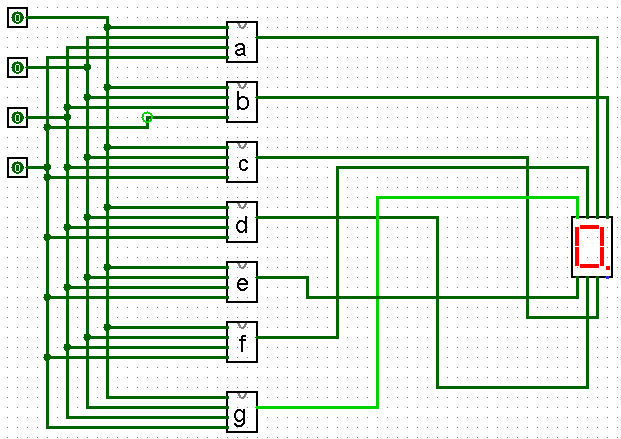
\includegraphics[width=\linewidth, keepaspectratio]{topLevelLogicCkt.png}
	\caption{Converter Top Level layout}
	\label{fig:TopLevelCkt}
\end{figure}

%Many of the gate level circuits use the inputs as well as their complements.  
%To reduce the number of gates in the final design, the inputs will each be inverted before being to the logic circuitry.  
%This will minimize redundancies in the gate layout.  
%This has not been included in this iteration of the design.


\section{Detailed Design}
\subsection{Gate Level} \label{sec:gateLevel}

The truth table for the converter, which includes its four inputs and seven outputs, is shown in Table \ref{tab:truthTable}.
A value of zero corresponds to the segment being on, and vice-versa.
From this, truth tables for each individual output were obtained and transferred to a program called Logisim, which is a free tool for designing and simulating logic circuits.
This tool was used to generate minimized NAND-only Boolean expressions for each module, as using only inverting logic will reduce the number of inverters required to realize the converter circuit.
Logisim was also used to generate the gate-level schematics for each module; the gate-level schematics for each module can be found in Appendix \ref{app:segmentLogic}, and the corresponding logic functions can be found in Appendix \ref{app:logicEquations}.

%The truth table for the four inputs and all seven outputs was created, it is shown in Figure \ref{fig:truthTable}.

\begin{table}[H]
	\centering
	\caption{Converter Truth Table}
	\vspace*{2mm}
	\label{tab:truthTable}
	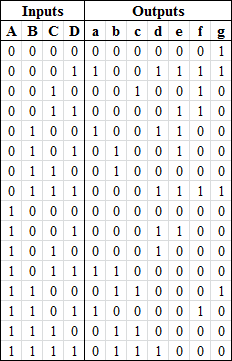
\includegraphics[width=0.4\linewidth, keepaspectratio]{hex7seg_truthTable.png}
\end{table}

\newpage
From the logic equations and gate-level schematics, note that the complement of any particular input is used many times.
In the actual implementation of the circuit, as opposed to what is shown in the gate-level schematics, the complements of the input signals will be produced only once and reused as needed, greatly reducing the number of inverters in the circuit.
Additionally, there are several terms in the logic equations that appear more than once: specifically $\overbar{(\bar{A}B\bar{C}\bar{D})}$, $\overbar{(AB\bar{C}D)}$, $\overbar{(AB\bar{D})}$, and $\overbar{(\bar{B}\bar{C}D)}$; the outputs of these gates will be reused as well.

To verify the functionality of the circuit, Logisim was used to simulate the output for each of the sixteen possible inputs.
The input and output waveforms were then plotted and are shown in Figure \ref{fig:BCD_sim}.
Comparing the simulated output to the converter circuit's truth table verifies that the design is valid.

%The truth table was transferred to the free software Logisim one output at a time.  
%Logisim analyzed the truth table for each output bit and generated a minimized NAND Boolean expression.  
%Utilizing inverting logic will reduce the number of inverters required to realize the circuit.
%Note that a zero in the output represents an active segment.
%The equivalent set of logic equations is shown in Appendix \ref{app:logicEquations}.

%Each logic equation represents a block on the top level diagram, and has a corresponding series of gates. The gate level design of these blocks is included in Appendix \ref{app:segmentLogic}.

\begin{figure}[H]
	\centering
	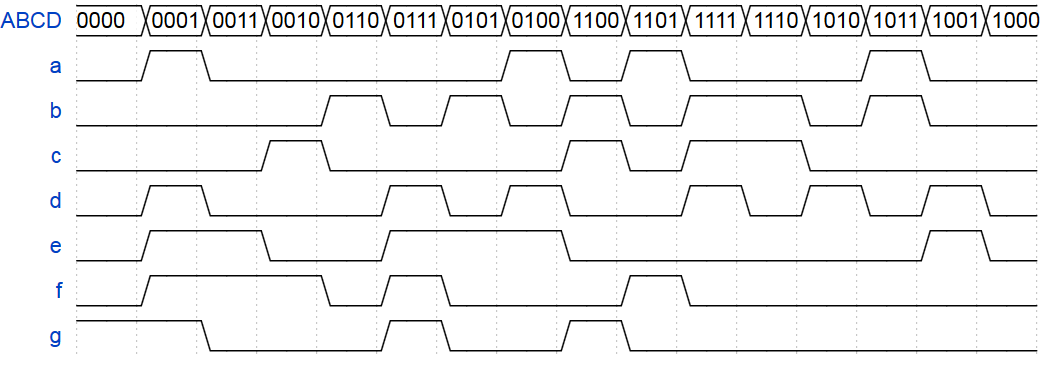
\includegraphics[width=\linewidth, keepaspectratio]{BCD_sim_waveform.png}
	\caption{Simulated Input and Output of Converter}
	\label{fig:BCD_sim}
\end{figure}

\subsection{Transistor Level}

\subsubsection{Transistor Level Schematics}

By using Logisim to implement each module with only NAND and inverter gates, the converter circuit can be realized with only a few gates: specifically two, three, and four input NAND gates, and an inverter.
Efficient implementations of these gates can be designed once and reused as needed, though different sizes of these gates will need to be made to optimize for delay and power consumption. 
The transistor level design of these gates is shown in Figures \ref{fig:2nandTran}, \ref{fig:3nandTran}, \ref{fig:4nandTran}, and \ref{fig:notTran}.
\begin{figure}[H]
	\centering
	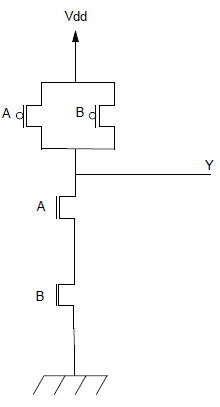
\includegraphics[width=0.3\linewidth, keepaspectratio]{NAND_2_Trans.png}
	\caption{Transistor Level Schematic for Two-Input NAND}
	\label{fig:2nandTran}
\end{figure}

\begin{figure}[H]
	\centering
	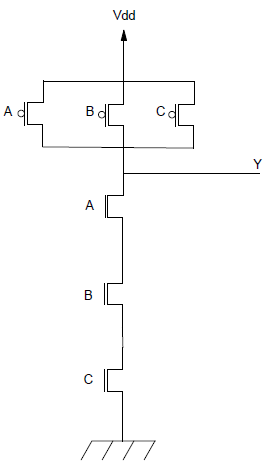
\includegraphics[width=0.3\linewidth, keepaspectratio]{NAND_3_Trans.png}
	\caption{Transistor Level Schematic for Three-Input NAND}
	\label{fig:3nandTran}
\end{figure}

\begin{figure}[H]
	\centering
	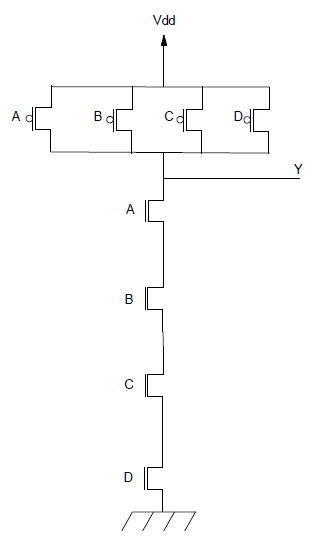
\includegraphics[width=0.3\linewidth, keepaspectratio]{NAND_4_Trans.png}
	\caption{Transistor Level Schematic for Four-Input NAND}
	\label{fig:4nandTran}
\end{figure}

\begin{figure}[H]
	\centering
	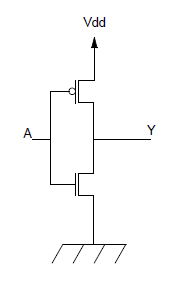
\includegraphics[width=0.3\linewidth, keepaspectratio]{NOT_Trans.png}
	\caption{Transistor Level Schematic for Inverter}
	\label{fig:notTran}
\end{figure}

\subsubsection{Transistor Sizing}
Sizing the transistors to optimize for delay first requires knowing the input and output capacitance for each module of the converter circuit. 
\todo{Output capacitance}
Since the circuit only generates inverted inputs once and reuses them, the input capacitance depends upon the largest fanout required for an inverted input. 
\todo{(relate fanout and transistor size)}
The required fanout for each inverted input is determined by counting the number of times each inverted term appears in the logic equations in Appendix \ref{app:logicEquations}, while accounting for terms appearing in the duplicate subcircuits mentioned in Section \ref{sec:gateLevel}.
Doing so yields fanouts for $\bar{A}$, $\bar{B}$, $\bar{C}$, and $\bar{D}$ of 11, 8, 8, and 6, respectively.
Each inverter will be sized so that it has the same driving strength as a unit-sized inverter with a fanout of one.
\todo{Inverter driving a NAND, so load cap is h*(kPMOS + kNMOS)*C, but what are the k values?}

When optimizing for delay, the input capacitance of interest is that of the critical path.
Since the inverter for $\bar{A}$ has the largest fanout it will have the largest input and output capacitance.
Since each module contains an $\bar{A}$ term, the critical path for each module will start with this inverter.


\newpage
\appendix
\section{Segment Logic Diagrams}
\label{app:segmentLogic}
% Segment a ==============================================
\subsection{Segment a}

\begin{figure}[H]
	\centering
	\label{fig:aBlockGates}
	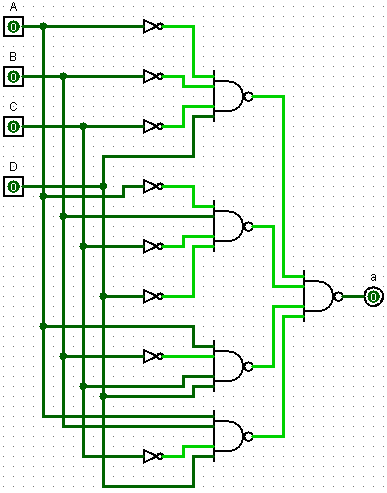
\includegraphics[width=0.5\linewidth, keepaspectratio]{a_logicCkt}
	\caption{Block a Gate Level Schematic}
\end{figure}

%Segment b ================================================
\subsection{Segment b}

\begin{figure}[H]
	\centering
	\label{fig:bBlockGates}
	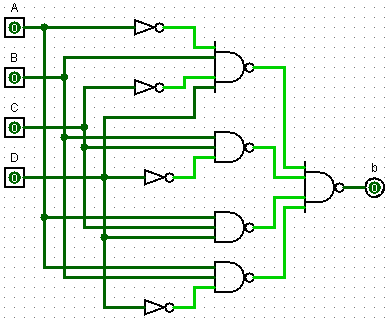
\includegraphics[width=0.5\linewidth, keepaspectratio]{b_logicCkt}
	\caption{Block b Gate Level Schematic}
\end{figure}

%Segment c ================================================
\subsection{Segment c}
\begin{figure}[H]
	\centering
	\label{fig:cBlockGates}
	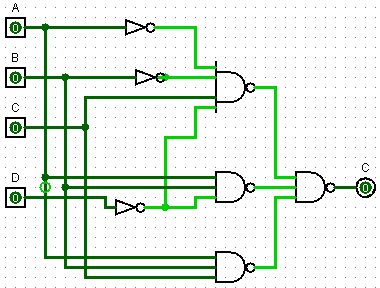
\includegraphics[width=0.5\linewidth, keepaspectratio]{c_logicCkt}
	\caption{Block c Gate Level Schematic}
\end{figure}

%Segment d =================================================
\subsection{Segment d}
\begin{figure}[H]
	\centering
	\label{fig:dBlockGates}
	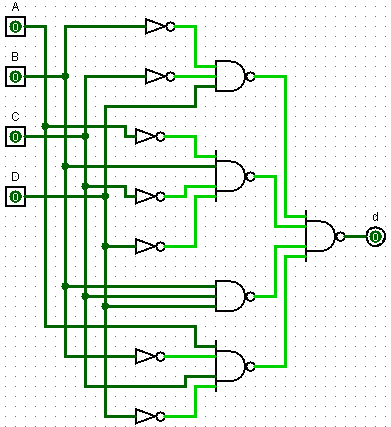
\includegraphics[width=0.65\linewidth, keepaspectratio]{d_logicCkt}
	\caption{Block d Gate Level Schematic}
\end{figure}

%Segment e ================================================
\subsection{Segment e}
\begin{figure}[H]
	\centering
	\label{fig:eBlockGates}
	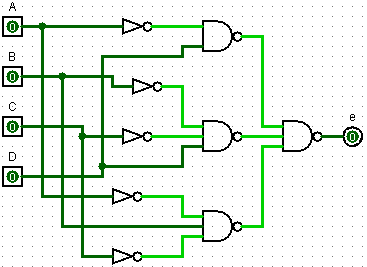
\includegraphics[width=0.65\linewidth, keepaspectratio]{e_logicCkt}
	\caption{Block e Gate Level Schematic}
\end{figure}

%Segment f ================================================
\subsection{Segment f}
\begin{figure}[H]
	\centering
	\label{fig:fBlockGates}
	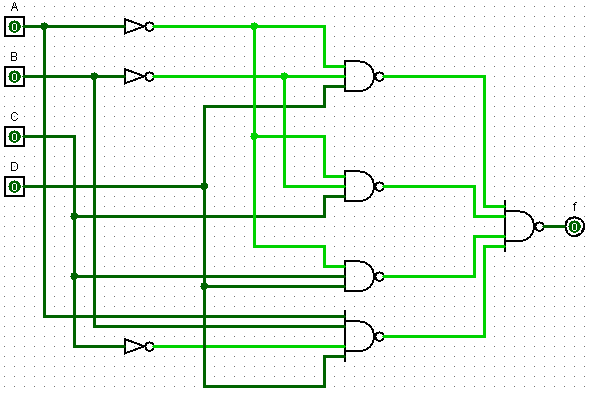
\includegraphics[width=0.65\linewidth, keepaspectratio]{f_logicCkt}
	\caption{Block f Gate Level Schematic}
\end{figure}

%Segment g ================================================
\subsection{Segment g}
\begin{figure}[H]
	\centering
	\label{fig:gBlockGates}
	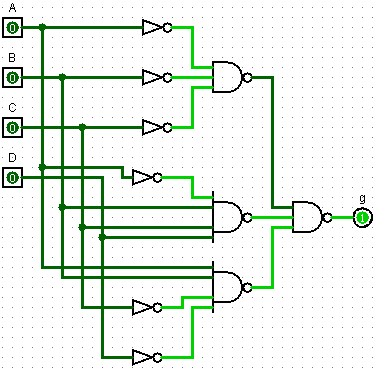
\includegraphics[width=0.65\linewidth, keepaspectratio]{g_logicCkt}
	\caption{Block g Gate Level Schematic}
\end{figure}


\newpage
\section{Logic Equations}
\label{app:logicEquations}
\begin{equation}
a = \overline{\overbar{(\bar{A}\bar{B}\bar{C}D)}\overbar{(\bar{A}B\bar{C}\bar{D})}\overbar{(A\bar{B}CD)}\overbar{(AB\bar{C}D)}}
\end{equation}

\begin{equation}
b = \overline{\overbar{(\bar{A}B\bar{C}D)}\overbar{(BC\bar{D})}\overbar{(ACD)}\overbar{(AB\bar{D})}}
\end{equation}

\begin{equation}
c = \overline{\overbar{(\bar{A}\bar{B}C\bar{D})}\overbar{(AB\bar{D})}\overbar{(ABC)}}
\end{equation}

\begin{equation}
d = \overline{\overbar{(\bar{B}\bar{C}D)}\overbar{(\bar{A}B\bar{C}\bar{D})}\overbar{(BCD)}\overbar{A\bar{B}C\bar{D}}}
\end{equation}

\begin{equation}
e = \overline{\overbar{(\bar{A}D)}\overbar{(\bar{B}\bar{C}D)}\overbar{(\bar{A}B\bar{C})}}
\end{equation}

\begin{equation}
f = \overline{\overbar{(\bar{A}\bar{B}D)}\overbar{(\bar{A}\bar{B}C)}\overbar{(\bar{A}CD)}\overbar{(AB\bar{C}D)}}
\end{equation}

\begin{equation}
g = \overline{\overbar{(\bar{A}\bar{B}\bar{C})}\overbar{(\bar{A}BCD)}\overbar{(AB\bar{C}\bar{D})}}
\end{equation}


\end{document}
